\documentclass[]{beamer}

\usepackage[utf8x]{inputenc}


% opciones para la presentacion
\usetheme{Warsaw}
% \usetheme{classic}



%datos de la presentacion
\title{Seguimiento de objetos en secuencias de imágenes RGB-D}
\subtitle{Tesis de licenciatura}
\institute{Facultad de Ciencias Exactas y Naturales}
\date[18/03/15]{Miércoles 18 de Marzo de 2015}
\author[Mariano Bianchi]{Mariano Bianchi}


\begin{document}

\maketitle
%--- Next Frame ---%


\section{Introduccion}
\begin{frame}[t]{Si nos organizamos...}
    \tableofcontents
    % comentar como va a estar organizada la charla
\end{frame}
%--- Next Frame ---%

\subsection{Motivación}
\begin{frame}{Aplicaciones} % si pongo la opcion [t] el texto empieza desde arriba
    % Permite generar estadísitcas deportivas midiendo la distancia recorrida por
    % jugadores de futbol, tiros al arco, goles, faltas realizadas, etc
    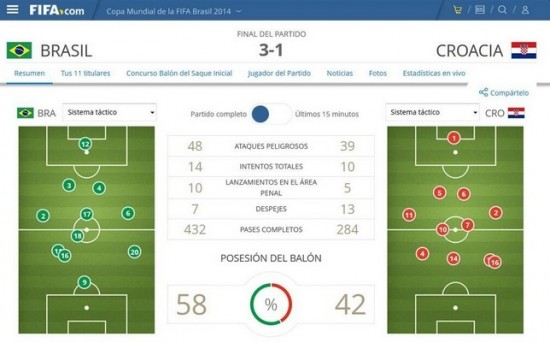
\includegraphics[scale=1]{img/estadistica.jpg}
\end{frame}

\begin{frame}{Aplicaciones}
    % Permite que un robot sepa de que manera tomar un objeto y usarlo como
    % herramienta de trabajo
    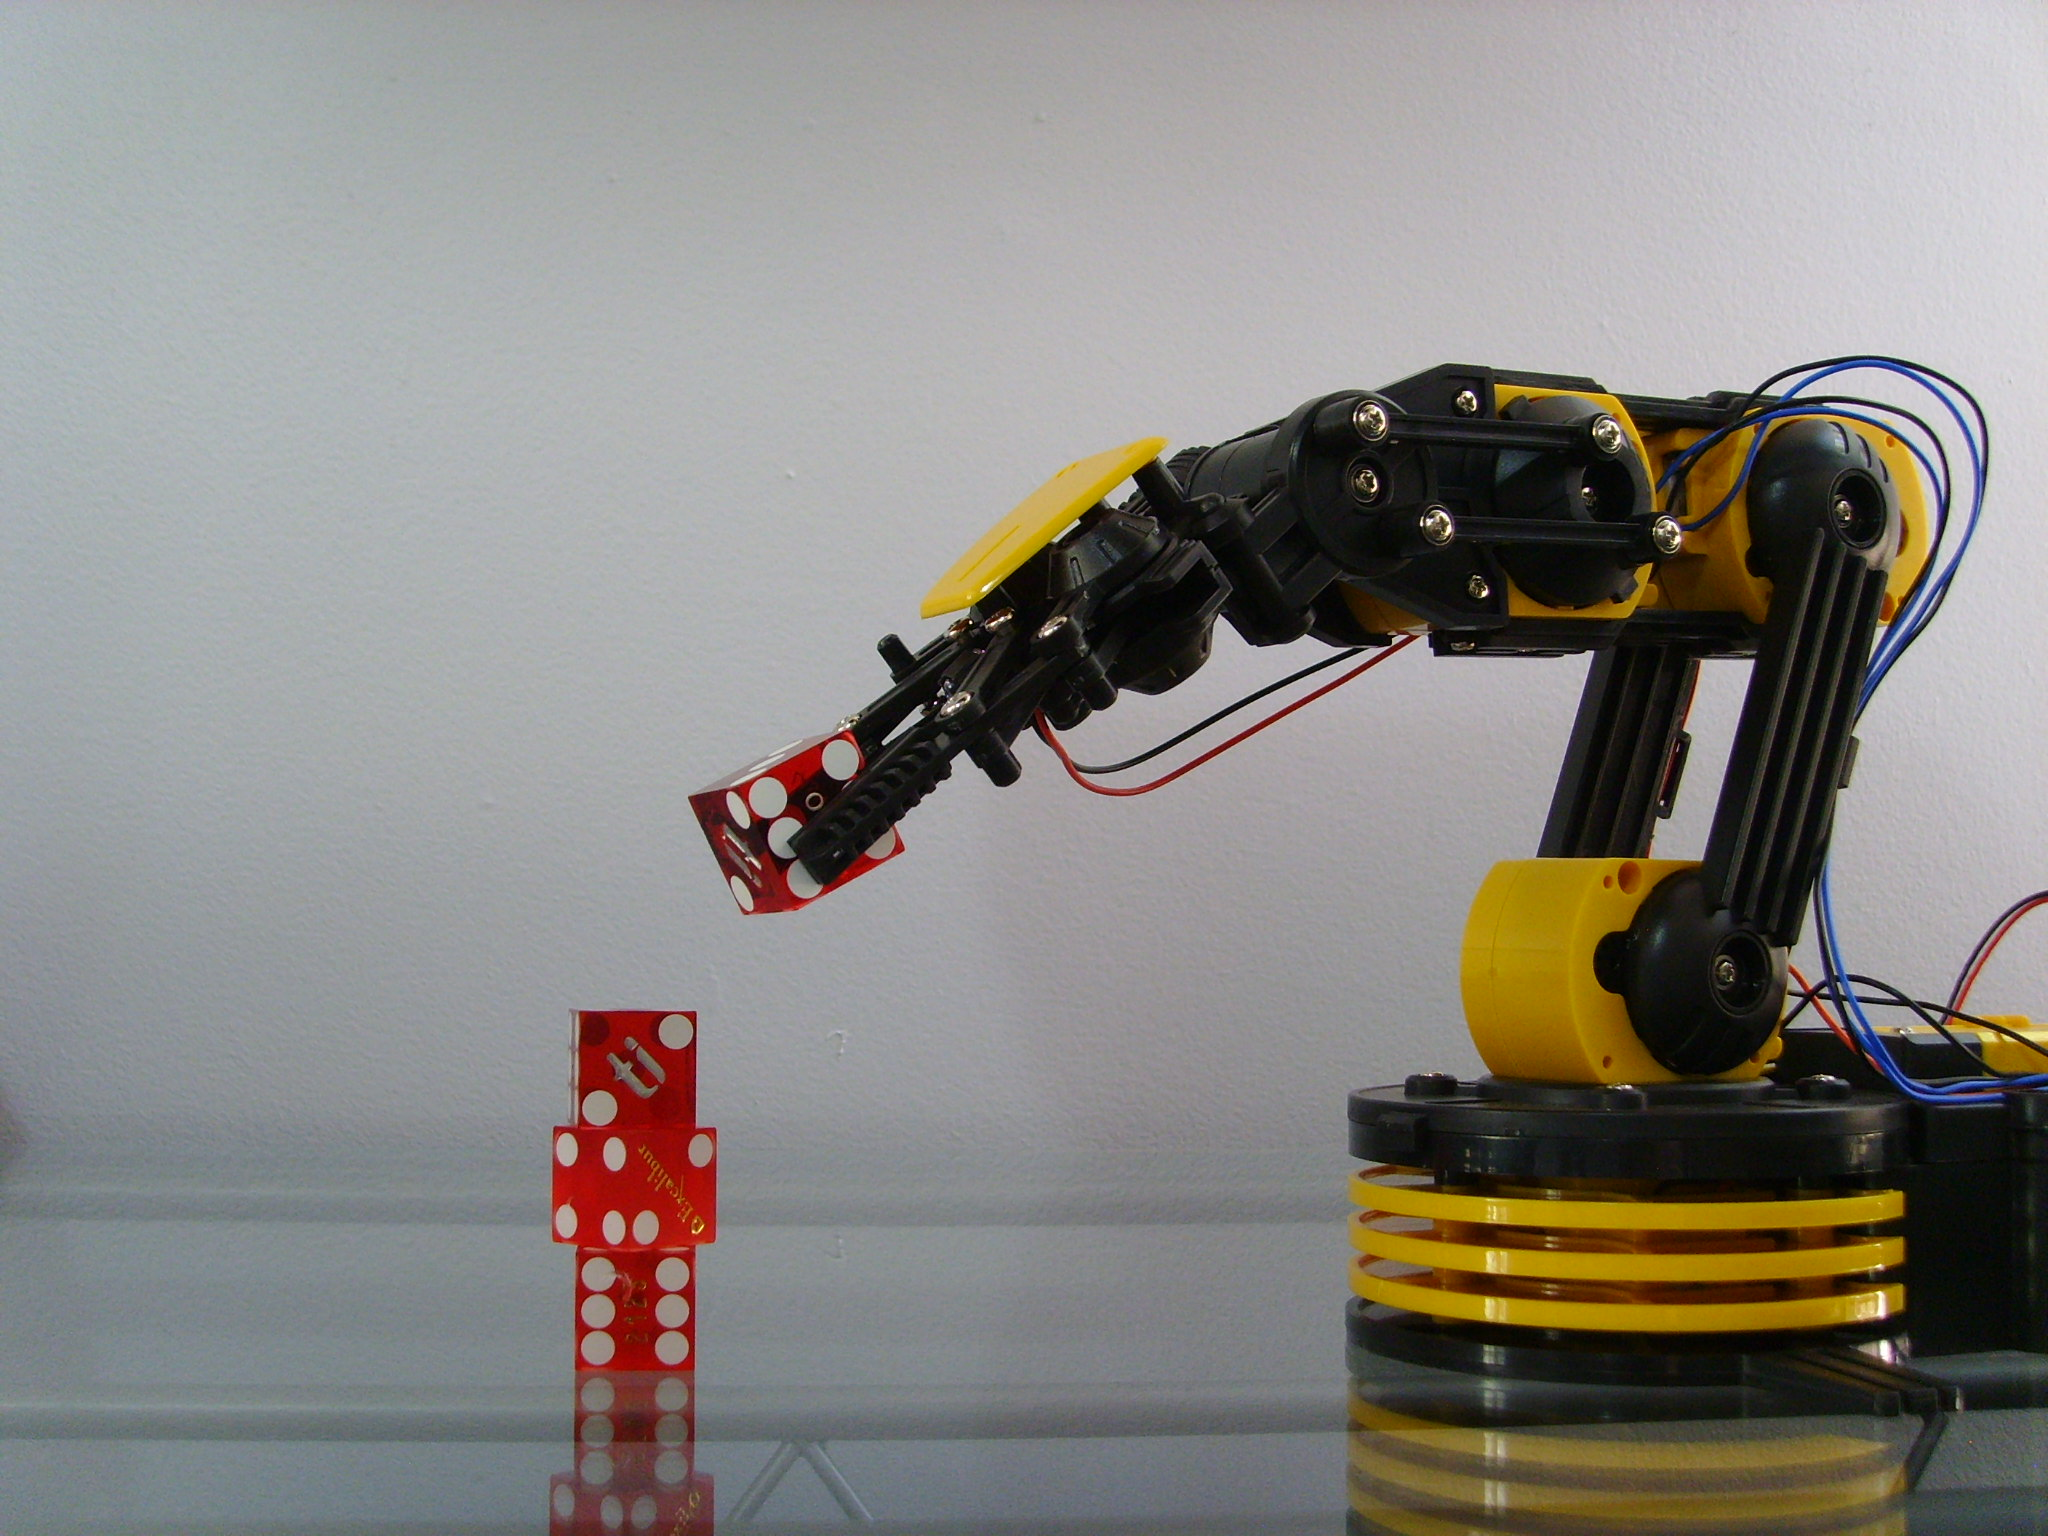
\includegraphics[scale=1]{img/robot.jpg}
\end{frame}

\subsection{Vamos por partes...(NO SE COMO LLAMAR A ESTO)}
\begin{frame}{Seguimiento}
    % El comportamiento esperado de un método de seguimiento es obtener para
    % cada imagen de una secuencia de imágenes o video, la ubicación de un
    % objeto en algún eje de coordenadas elegido. Por ejemplo, lo de la imagen
    IMAGEN DE UN FRAME CON EL OBJETO EN UN RECUADRO Y MARCANDO LAS COORDENADAS
    DE LOS PIXELES QUE LO DESCRIBEN
\end{frame}
%--- Next Frame ---%


\begin{frame}{Imágenes RGB-D}
    Una imagen RGB-D está compuesta por dos partes. Una de ellas es una
    imagen RGB
    % Las imágenes RGB son las más comunes y que todos conocen. Es simplemente
    % una fotografía. RGB significa Red Green Blue, que son los colores
    % primarios lumínicos (en el dominio de la luz), es decir, que el resto de los colores puede definirse
    % con una combinación de estos tres colores
    \begin{block}
        PEGAR UNA IMAGEN RGB CUALQUIERA
    \end{block}
\end{frame}
%--- Next Frame ---%


\begin{frame}{Información de profundidad}
    % Un sensor RGB-D cuenta con una cámara tipo webcam que otorga imagenes RGB,
    % un proyector infrarrojo
    \begin{block}
        MOSTRAR SENSOR RGB-D, contar como funciona y mostrar con el pcl_viewer una nube de puntos
    \end{block}
\end{frame}
%--- Next Frame ---%


    \begin{itemize}
        \item
        \item motivacion
        \item explicar parte por parte que significa el título de la tesis
        \begin{itemize}
            \item seguimiento
            \item objeto
            \item secuencia de imagenes
            \item rgb-d (sensores, imagenes)
        \end{itemize}
        \item esquema de seguimiento
        \item objetivos, remarcando el aporte
    \end{itemize}
\end{frame}
%--- Next Frame ---%


\section{Desarrollo}
\begin{frame}{Desarrollo}
    \begin{itemize}
        \item motivaciones, por que la separacion de los metodos, comparar metodos rgb y d
        \item explicacion de los métodos, con ejemplos en imagenes
        \item algun video de ejemplo sobre lo que se espera del sistema
    \end{itemize}

\end{frame}
%--- Next Frame ---%


\section{Resultados}
\begin{frame}{Resultados}
    \begin{itemize}
        \item base de datos
        \item objetos y escenas elegidos para seleccion de parametros
        \item seleccion/exploracion de parametros
        \item analisis sobre los metodos
        \item resultados por método y del sistema
        \item resultados del sistema con nuevos objetos
    \end{itemize}
\end{frame}
%--- Next Frame ---%

\section{Conclusiones y trabajo a futuro}
\begin{frame}{Conclusiones y trabajo a futuro}
    \begin{itemize}
        \item conclusiones
        \item mejoras a implementar
    \end{itemize}
\end{frame}
%--- Next Frame ---%


\end{document}
